\chapter{光の量子状態}

本章では、まず、光を調和振動子の集まりとして考える手続きについて述べる。その後、代表的な光の量子状態である、光子数状態、コヒーレント状態、スクイズド状態を説明する。特に、これらが複素振幅や光子数についてどのような揺らぎを有するのかを説明する。

\section{量子光学の手続き}
量子光学では、以下のような手続きで、光を調和振動子に対応させる。

まず、光を色々な空間モード、周波数モード、偏光に分解する。その分解の仕方に関してはひとつに決まっているわけではない\footnote{その理屈は、正規直交基底の取り方が複数あるのと同じである。分解の仕方によって計算結果が変わってくるわけではない。}。

例えば、レーザからビーム状の光が出力されている状況を考えよう。このレーザビームの空間分布は非常に安定している、すなわち横モードがシングルモードであるとし、また、偏光は単一であるとする。このビームが進む方向を$z$方向とし、時間$-\Delta t/2 \leq t < \Delta t/2$において$z = 0$を通過する光について考えるものとする。

この時間における光電界の時間波形を$s(t)$とし、$s(t)$のフーリエ変換$S(\omega)$を考えよう。以下のように$S(\omega)$は角周波数$\Delta \omega = 2\pi / \Delta t$間隔のスペクトルからなることがわかる\footnote{ここに書いてあることは、要は「各空間モード・周波数モードは複数の基底の線型結合で表現できて、全ての基底に対する複素振幅を決めれば元の波形を表現できるよ」ということだけであるので読み飛ばしても構わない。なお、このときの基底の数のことを「自由度」という。}。

まず、$s(t)$を周期関数化した$s_1(t) = \sum_{m = -\infty}^{\infty}s(t-m\Delta t)$を考える。$s_1(t)$のフーリエ変換$S_1(\omega)$は周期関数のフーリエ変換であるから、
角周波数$\Delta \omega = 2\pi/\Delta t$の離散スペクトルから構成される。ここで、$s(t) = s_1(t)\mathrm{rect}(t / \Delta t)$である\footnote{$\mathrm{rect}(t)$は$(|t|<1/2)$の時1、それ以外で0を取る関数である。}から、$S(\omega)$は、$S_1(\omega)$に$\mathrm{rect}$関数のフーリエ変換である$\mathrm {sinc}$関数を畳み込んだものである。このように考えると、$S(\omega)$の自由度は、離散スペクトルの自由度と等しく、周波数帯域を$\Omega$とすれば、$\Omega/\Delta\omega$個の複素数(フーリエ係数)で$s(t)$を表すことができる。

このとき、$\Delta t$の値を2倍にすると、離散スペクトルの周波数間隔$\Delta \omega$が半分になるので、自由度の数は2倍になる。これは、計測時間$\Delta t$を保ったまま、2回計測を行ったときの自由度の数と同じである。このことから想像できるように、時間波形をフーリエ変換してスペクトル分解する際は、$\Delta t$の切り方をどのようにしても良い。時間幅$\Delta t$と周波数帯域$\Omega$が決まれば、その自由度は$\Omega\Delta t/2\pi$個となる。

実際には、$\Delta t$は考えやすい値に設定することが多い。例えば、光ファイバ通信においては1ビットの光に1つの自由度を設定したり、光パルスであれば1つの光パルスに1つの自由度を設定する等である。もちろん、1つの光パルスの中で強度や位相が変化する場合などは、複数の自由度を考える必要がある。いずれにせよ、このようにして、時間・周波数領域で複数の自由度に分解することができる。

光の周波数が決まれば、複数の空間モードに展開することができる。その展開の仕方も、正弦波(平面波)で展開する方法、エルミートガウスモードで展開する方法など様々な方法が考えられる。ただ、ここでは簡単のため、空間モードは単一であるとしよう。シングルモード光ファイバー中の光や、単一横モードのレーザーの出力を考えるときにはこれで十分である。

一旦、このようにモードに分解できたら、その単一のモードに注目する。時間$\Delta t$の間に光が進む距離は$L = c\Delta t/n$であるから、その間の光が持つエネルギーは、
\begin{equation}
U = \frac 1 2 \int_V \left(\varepsilon E^2 + \mu H^2\right)dr = \int_V \varepsilon E^2 dr
\end{equation}
と求められる。ここで、$\frac 1 2 \varepsilon E^2$は電界が有する単位体積あたりのエネルギー、$\frac 1 2 \mu H^2$は磁界が有する単位体積あたりのエネルギーであり、電界と磁界のエネルギーが等しいことを用いた。また、$V$は空間モードの体積である。

%\textbf{この辺り怪しい。式(3.3)は教科書通りだが。。。$p^2/2$は運動エネルギーで、その時間平均は$p^2/4$となる。$(1/2)\varepsilon E^2$は電場のエネルギーで、それを空間$V$で平均すると$(1/4)\varepsilon V E^2$になる。磁場のエネルギーはこれと同じ。$p^2/4$と$(1/4)\varepsilon V E^2$}

%単純に、$(1/2)\varepsilon VE^2$を$(1/2)p^2$に対応させれば良いはず。

量子光学では、このひとつのモードを、同じエネルギーを有する調和振動子に対応させる。慣例的に、$E \propto -p$となるようにすることが多い
\footnote{これは、場の量子論においてベクトルポテンシャル$\pmb A$の一つのモードを調和振動子の位置$q$に対応させるためである。理論的には、電界$E$を$q$に対応させても$p$に対応させても、調和振動子の位相が異なるだけなので何の問題も生じないが、ここでは物理系の流儀に合わせてこのような定義を採用する。}。
$E$の振幅が空間的に一様であるとすれば、$U = \frac 1 2 \varepsilon V E^2$であり、これが運動エネルギー$\frac 1 2 p^2$と一致するようにするため、$t = 0$、$z = 0$において
\begin{equation}
  E = -\frac 1 {\sqrt {\varepsilon V}}p
\end{equation}
とおく。ここで、$E$と$p$を演算子で表すと、次式を得る。
\begin{equation}
  \hat E = -\frac 1 {\sqrt{\varepsilon V}}\hat p = i\sqrt{\frac{\hbar \omega}{2\varepsilon V}}(\hat a - \hat a^\dagger)
\end{equation}
$\hat E$の$t$および$z$の依存性は、演算子をハイゼンベルグ描像で時間発展及び空間発展させることで次式のように表せる。
\begin{equation}
  \hat E(x,y,z,t) = i\sqrt{\frac{\hbar \omega}{2\varepsilon V}}(\hat a e^{i(kz-\omega t)} - \hat a^\dagger e^{-i(kz-\omega t)})
\end{equation}

なお、この式は、電場が空間的に一様であるという仮定を置いた近似式である。本来は、ビームの空間分布を考え、位置によって電場の大きさや位相が異なることを表さなければならない。とはいえ、そのような取り扱いをしたとしても、ひとつの空間モードを調和振動子として表すことに変わりないので、ここではこれ以上深入りしない。

各モードを調和振動子に対応させられることがわかったので、次は、光(量子的調和振動子の)の代表的な量子状態である、光子数状態、コヒーレント状態、スクイズド状態について説明する。これらの量子状態は、対応する状態ベクトル$\ket \phi$で表される。

$\ket \phi$の性質を知るには、この状態に対して物理量の計測を行った時の期待値を計算していけば良い。前章で述べたように、物理量$\hat A$と状態ベクトル$\ket \phi$が決まれば、物理量の期待値を計算することができる。ここで用いる物理量としては、光子数$\hat n = \hat a^\dagger \hat a$, $\hat a$の実部$\hat a_1 = \frac{1}{2}(\hat a + \hat a^\dagger) = \frac{1}{\sqrt 2}\hat Q$, および$\hat a$の虚部$\hat a_2 = \frac{1}{2i}(\hat a - \hat a^\dagger$)等がある。


\section{光子数状態}

$\ket \phi$が$\ket 0, \ket 1, \ket 2, \ket 3, \hdots$のいずれかである時、これは光子数が一意に決まった状態であるから、光子数状態という。光子数状態$\ket n$に対する光子数の期待値は、
\begin{equation}
  \braket{n|\hat a^\dagger \hat a|n} = n\braket{n|n} = n
\end{equation}
である。また、光子数の分散は、
\begin{equation}
\braket{n|(\hat a^\dagger \hat a)^2|n} - n^2 = n\braket{n|\hat a^\dagger \hat a|n} - n^2 = n^2 - n^2 = 0  
\end{equation}
となる。このように、光子数状態では光子数が確定しており、そのゆらぎはない。

次に、実部$\hat a_1$を見てみよう。その期待値は、
\begin{equation}
\begin{aligned}
  \braket{n|\hat a_1|n} &= \braket{n|\frac{\hat a + \hat a^\dagger}{2}|n} = \frac 1 2 \braket{n|\hat a|n} + \frac{1}{2}\braket{n|\hat a^\dagger|n}\\
  &= \frac{\sqrt n}{2}\braket{n|n-1} + \frac{\sqrt{n + 1}}{2}\braket{n|n+1} = 0
\end{aligned}
\end{equation}
であり、また、分散は、平均が0であることから2乗の平均と等しく、
\begin{equation}
\begin{aligned}
  \braket{n|\hat a_1^2|n} &= \frac{1}{4}\braket{n|\hat a\hat a+\hat a \hat a^\dagger + \hat a^\dagger \hat a + \hat a^\dagger \hat a^\dagger|n} \\
  &= \frac{1}{4}\braket{n|\hat a \hat a^\dagger + \hat a^\dagger \hat a|n}\\
  &= \frac{1}{4}\braket{n|2\hat a^\dagger \hat a + 1|n} = \frac{1}{2}\left(n + \frac 1 2\right)  
  \label{eq:variance_Fock_real}
\end{aligned}
\end{equation}
を得る。同様に、虚部$\hat a_2$に対しても、
\begin{equation}
  \braket{n|\hat a_2|n} = 0
\end{equation}
\begin{equation}
  \braket{n|\hat a_2^2|n} = \frac{1}{2}\left(n + \frac 1 2\right)
  \label{eq:variance_Fock_imag}
\end{equation}
が成り立つ。

式(\ref{eq:variance_Fock_real})(\ref{eq:variance_Fock_imag})は、$n = 0$においても、複素振幅の実部、虚部がゆらぎを持つことを表している。このゆらぎのことを\textbf{真空場ゆらぎ}という。
真空場は、図\ref{fig:vacuum_field}に示すイメージ図のように、複素振幅の実部・虚部に1/4の分散を有する。この2つの分散の和が1/2であることは、基底状態$\ket 0$のエネルギーが$\frac 1 2 \hbar \omega$であることと対応している。
%\footnote{$\ket 1, \ket 2, \hdots$が複素平面上でどのような分布を取るかは付録に示す。}

\begin{figure}
  \centering
  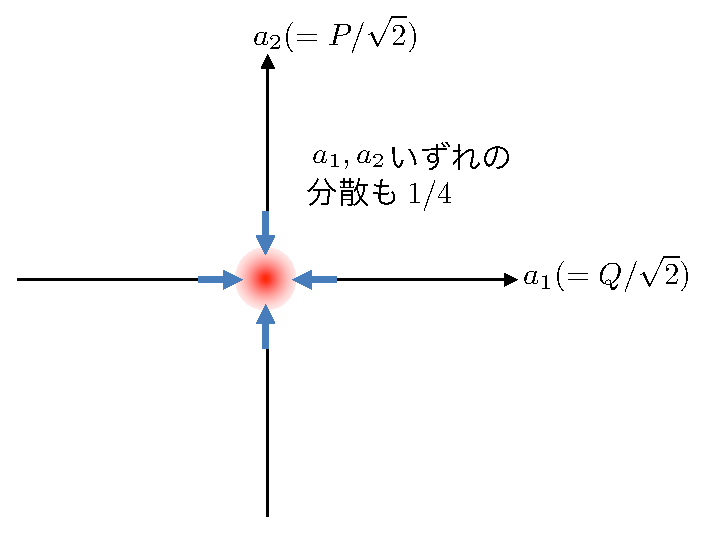
\includegraphics[width=8cm]{fig/3-1_vacuum.eps} 
  \caption{真空場の複素振幅のイメージ。}
  \label{fig:vacuum_field}
\end{figure}

また、光子数状態は光の波動としての位相の情報を持たない。古典的な波動は、周波数$\omega$で時間変化し、その変化のタイミングが位相に対応する。一方、光子数状態はハミルトニアン(時間発展演算子)の固有状態であり、時間とともに変化をしない状態である。ただ、計測される光子数は一意に決まり、計測される複素振幅にはゆらぎがある。

なお、厳密な光子数状態を作るのは技術的に大変難しいが、最近では量子ドット等を用いて光子数状態を発生させることができつつあり、量子暗号等への応用が期待されている。

また、光子数状態は正規直交系であり、光子数状態以外の量子状態は、複数の光子数状態の重ね合わせとして表される。これが、検出される光子数のばらつきに対応する。


\begin{comment}
\subsubsection{光子数状態の重ね合わせ}
光子数状態は時間とともに変化しない状況であった。一方、異なる光子数状態を重ね合わせると、時間とともに変化する量子状態を作ることができる。

例として、$\ket \phi = \frac{1}{\sqrt 2}(\ket 0 + \ket 1)$を考えてみよう\footnote{$\frac{1}{\sqrt 2}$のファクタは、規格化($\braket{\phi|\phi} = 1$)のためにつけた。}。シュレディンガー描像では、エネルギー$E_n = \frac{1}{2}(n + 1/2)$を有するエネルギー固有状態は角周波数$\omega_n = E_n / \hbar = \omega (n + \frac 1 2)$で時間発展する。また、したがって、
\begin{equation}
\begin{aligned}
  \ket {\phi (t)} &= \frac 1 {\sqrt 2}\left(\ket 0 e^{-i\omega (1/2)} + \ket 1 e^{-i\omega (1 + 1/2)}\right)\\
  &= \frac{e^{-i\omega t/2}}{\sqrt 2}\left( \ket 0 + \ket 1 e^{-i\omega t}\right)
\end{aligned}
\end{equation}
を得る。$t = 0$では$\ket{\phi(0)} \propto {\ket 0 + \ket 1}$, $t = \pi/\omega$では$\ket{\phi(\pi/\omega)} \propto {\ket 0 - \ket 1}$となり、時間発展とともにこれを繰り返すことがわかる。
$\ket 0$、$\ket 1$の$Q$表示(図?)を考えると、$\ket 0 = \ket 1$は、波動関数の分布が$+Q$の方向に偏っている一方、$\ket 0 - \ket 1$は$-Q$の方向に偏っている。このように、異なる光子数状態を重ね合わせることで、周波数$\omega$で振動する光を表すことができる。
\end{comment}

\section{コヒーレント状態}
複数の光子数状態の重ね合わせとして次式で表される状態を\textbf{コヒーレント状態}という。
\begin{equation}
  \ket \alpha = \exp \left( -\frac{|\alpha|^2}{2} \right)\sum_{n = 0}^{\infty}\frac{\alpha^n}{\sqrt{n!}} \ket n
  \label{eq:coherent_state}
\end{equation}
コヒーレント状態はレーザーでつくられる正弦波的な波動に対応する量子状態であり、複素振幅$\alpha$を有し、また、振幅及び光子数のゆらぎを有する。

式(\ref{eq:coherent_state})の右辺のうち、コヒーレント状態の性質を決める重要な項は$\ket n$の線形結合を取っている部分である。一方、$\exp$の部分は、$\braket {\alpha|\alpha} = 1$とするための規格化因子である。

以下では、コヒーレント状態が持つ幾つかの性質を見ていこう。

\subsection{消滅演算子の固有状態}
$\ket \alpha$は、消滅演算子$\hat a$の固有状態であることが知られている。このことは以下のように示される。
\begin{equation}
\begin{aligned}
	  \hat a \ket \alpha &= \exp\left(-\frac{|\alpha|^2}{2}\right)\sum_{n = 0}^\infty \frac{\alpha^n}{\sqrt{n!}}\sqrt n \ket{n - 1}\\
	  &=\alpha \exp\left(-\frac{|\alpha|^2}{2}\right)\sum_{n = 1}^\infty\frac{\alpha^{n - 1}}{\sqrt{(n - 1)!}}\ket{n - 1}\\
	  &=\alpha \ket \alpha
\end{aligned}
\end{equation}
なお、2行目で和が$n = 1$から始まっているのは、$\hat a\ket 0 = 0$であることを利用したためである。
また、このエルミート共役を取ると、$\bra \alpha \hat a^\dagger = \alpha^* \bra \alpha$である。

なお、$\hat a$がエルミート演算子でない($\hat a^\dagger \neq \hat a$)ことに注意が必要である。このため、$\ket \alpha$は$\hat a$の固有状態ではあるが、$\alpha$を誤差なく直接測定することはできない。また、固有状態$\ket \alpha$は正規直交基底にはなっていない。これらの性質は後に述べる。

\subsection{光子数の分布}
コヒーレント状態で$n$個の光子を検出する確率を$P(n)$とする。$P(n)$を求めるには、光子数状態$\ket n$との内積を取り、そのノルムを求めればよいから、次式のように計算できる。
\begin{equation}
\begin{aligned}
  P(n) &= |\braket {n | \alpha}|^2 = \left| \exp\left(-\frac{|\alpha|^2}{2}\right) \frac{\alpha^n}{\sqrt{n!}}\right|^2\\
  &= \exp \left(-|\alpha|^{2}\right)\frac{|\alpha|^{2n}}{n!}\\
  &\equiv \exp \left(-\lambda\right)\frac{\lambda^n}{n!}
\end{aligned}
\end{equation}
ただし、3行目で$\lambda = |\alpha|^2$とおいた。このように、コヒーレント状態の光子数の分布はポアソン分布となる。

コヒーレント状態は、光が波動でありながらも、光子が確率的に到来し、ショット雑音を生むことを表している。

\subsection{複素振幅の期待値と分散}
複素振幅の演算子である$\hat a$はエルミートでないのでその測定を行うことはできない。しかし、複素振幅の実部を
\begin{equation}
  \hat a_1 = \frac 1 2 (\hat a + \hat a^\dagger)
\end{equation}
と定義すれば、$\hat a_1^\dagger = \hat a_1$より$\hat a_1$はエルミートであるから、その測定を行うことができる。同様に、複素振幅の虚部を
\begin{equation}
  \hat a_2 = \frac 1 {2i} (\hat a - \hat a^\dagger)
\end{equation}
と定義すれば、$\hat a_2$も同様にエルミートとなり、その測定が可能である。

コヒーレント状態$\alpha$に対して、複素振幅の実部$\hat a_1$の期待値と分散を求めよう。なお、ここでは$\braket{\alpha|\hat a_1|\alpha} \equiv \braket{\hat a_1}$のように表すこととする。
\begin{equation}
\begin{aligned}
  \braket{\hat a_1} &= \frac{1}{2}\braket{\alpha|\hat a + \hat a^\dagger|\alpha} = \frac{1}{2}\braket{\alpha|\hat a |\alpha} + \frac{1}{2}\braket{\alpha|\hat a^\dagger |\alpha}\\
  &= \frac{1}{2}\alpha \braket{\alpha|\alpha} + \frac{1}{2} \alpha^* \braket{\alpha|\alpha} = \frac 1 2 (\alpha + \alpha^*) = \mathrm{Re} \ \alpha
\end{aligned}
\end{equation}

\begin{equation}
\begin{aligned}
  \braket{\hat a_1^2} &= \frac{1}{4}\braket{\alpha|(\hat a + \hat a^\dagger)^2|\alpha} = \frac{1}{4}\braket{\alpha|\hat a \hat a + \hat a \hat a^\dagger + \hat a^\dagger \hat a + \hat a^\dagger \hat a^\dagger|\alpha}\\
  &= \frac 1 4 \braket{\alpha|\hat a \hat a + 2\hat a^\dagger \hat a + 1 + \hat a^\dagger \hat a^\dagger|\alpha}\\
  &= \frac{1}{4}\left\{\alpha^2 + 2|\alpha |^2 + 1 + (\alpha^*)^2\right\}
\end{aligned}
\end{equation}
\begin{equation}
	\begin{aligned}
		\braket{\hat a_1^2} - \braket{\hat a _1}^2 &= \frac{1}{4}\left\{\alpha^2 + 2|\alpha |^2 + 1 + (\alpha^*)^2\right\} - \frac{1}{4}\left\{\alpha^2 + \alpha \alpha^* + \alpha^*\alpha + (\alpha^*)^2\right\} = \frac 1 4
	\end{aligned}
\end{equation}
したがって、コヒーレント状態$\ket \alpha$の複素振幅の実部$\hat a_1$を計測すると、その平均値は$\mathrm {Re} \ \alpha$、分散が$\frac 1 4$であることがわかる。

同様に、虚部$\hat a_2$を計測すると、その平均値は$\mathrm{Im} \ \alpha$、分散が$\frac 1 4$であることを示すことができる。この分散は真空状態$\ket 0$の分散と同じである。

この様子を元に、$\ket \alpha$を複素平面のように表したものを図\ref{fig:coherent_state}に示す。$(\mathrm {Re} \ \alpha, \mathrm{Im} \ \alpha)$を中心として、実部、虚部にいずれも1/4の分散を有するように描いている。このように、広がりのある複素振幅が、時間発展とともに$e^{-i\omega t}$のように回転していく。実部に注目すると、広がりを持ったまま正弦波で振動しており、虚部に注目しても同様である。このように、コヒーレント状態は、調和振動子の複素振幅が広がりを持ったまま時間発展する様子と考えることができる。

一方、このような図を解釈するときには注意が必要である。なぜなら、$\hat a_1$と$\hat a_2$は同時に測定できないためである。($[\hat a_1, \hat a_2] = i/2$である。)
\begin{figure}
  \centering
  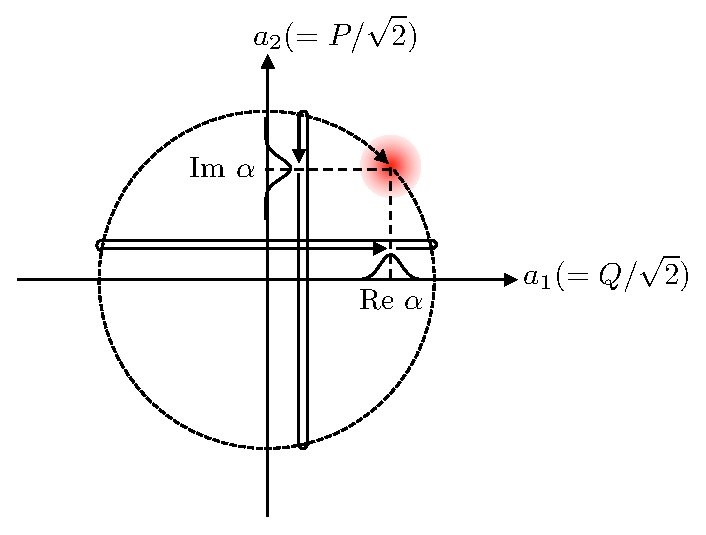
\includegraphics[width=8cm]{fig/3-2_coherent_state.eps} 
  \caption{コヒーレント状態の複素振幅のイメージ。複素振幅の実部$a_1$の中心はRe $\alpha$、虚部$a_2$の中心はIm $\alpha$にあり、その分散は真空場と同じ1/4である。シュレディンガー描像で時間発展すると、$a_1$の分布と$a_2$の分布のいずれも正弦波状に振動する。このとき、$a_1$と$a_2$の分布($\hat a_1$と$\hat a_2$は同時に計測できないことに注意)は、$a_1-a_2$平面上で回転する。}
  \label{fig:coherent_state}
\end{figure}

\subsection{変位演算子によるコヒーレント状態の生成}
前節で見たように、コヒーレント状態は、その複素振幅の分散が真空場$\ket 0$と同じであり、複素振幅が$\alpha$であるような状態である。このことに注目すると、$\ket 0$に対して複素振幅を少しずつ変化させていく操作を加えると、コヒーレント状態を生成することができる。

このように、複素振幅を変化させる演算子を変位演算子といい、次式で与えられる。
\begin{equation}
  \hat D(\alpha) = \exp(\alpha \hat a^\dagger - \alpha^*\hat a)
\end{equation}
変位演算子はユニタリ演算子であり、これを用いて、
\begin{equation}
  \ket \alpha = \hat D(\alpha)\ket 0
\end{equation}
であることを示すことができる。この証明には、Baker-Cambell-Hausdorffの公式と呼ばれるものを用いる。これは、$[\hat A, [\hat A, \hat B]] = [\hat B, [\hat A, \hat B]] = 0$のとき、$\exp(\hat A + \hat B) = \exp \hat A \exp \hat B \exp \left(-\frac{1}{2} [\hat A, \hat B]\right)$が成り立つ、というものであり、これに$\hat A = \alpha \hat a^\dagger$、$\hat B = -\alpha^*\hat a$とすれば左辺は$\hat D(a)$となる。ここで$\hat D(\alpha) \ket 0$を計算すると、式(\ref{eq:coherent_state})を得る。

とはいえ、この証明はあまり直感的でないので、ここでは少し違う観点から変位演算子の働きを調べておこう。演算子$\hat H = i\hbar(\alpha\hat a^\dagger - \alpha ^*\hat a)$を考えると、これは$\hat H^\dagger = \hat H$であることから、エルミートであることがわかる。これをハミルトニアンとする時間発展演算子を考える\footnote{ここでの$t$はもはや時間ではなく、ケットベクトルを徐々に変化させるためのパラメータである。}と、
\begin{equation}
\hat U(t) = \exp\left(\frac{t}{i\hbar}\hat H\right) = \exp\left\{t(\alpha\hat a^\dagger - \alpha^* \hat a)\right\}
\end{equation}
であるから、$\hat U(1) = \hat D(\alpha)$である。
ここで、$t = 0 \to 1$で$\hat a$, $\hat a^\dagger$が$\hat a'$, $\hat a'^\dagger$に変化すると考えよう。ハイゼンベルグの運動方程式から、
\begin{equation}
 \frac{d}{dt}\hat a = \frac i \hbar[\hat H, \hat a] = -\alpha [\hat a^\dagger, \hat a] = \alpha
\end{equation}
\begin{equation}
  \frac{d}{dt}\hat a^\dagger = \frac i \hbar [\hat H, \hat a^\dagger] = \alpha^*[\hat a, \hat a^\dagger] = \alpha^*
\end{equation}
したがって、
\begin{equation}
  \hat a' = \hat a + \alpha
\end{equation}
\begin{equation}
  \hat a'^\dagger = \hat a^\dagger + \alpha ^*
\end{equation}
である。これは、ある状態ベクトルに変位演算子$\hat D(\alpha)$を作用させると、複素振幅が$\alpha$だけ変化することを表している。

\subsection{ショット雑音と真空場}
コヒーレント状態は直感的に「複素振幅$\alpha$の周りに真空場があるもの」と捉えることができる。コヒーレント状態の平均の光子数は
\begin{equation}
  \braket{\hat n} = \braket{\alpha | \hat n |\alpha} = \braket {\alpha |\hat a^\dagger \hat a|\alpha} = |\alpha|^2
\end{equation}
である。したがって、
\begin{equation}
  |\alpha| = \sqrt{\braket {\hat n}}
\end{equation}
である。また、コヒーレント状態において複素振幅の実部・虚部のいずれも1/4の分散を有しており、その標準偏差は$\sqrt{1/4} = 1/2$である。このことから、$|\alpha|$の標準偏差も1/2である\footnote{半径方向の標準偏差が実部の標準偏差と等しいことは、コヒーレント状態を時間発展させて複素振幅が実数になった瞬間の広がりを考えると理解できる。}。

このことから、複素振幅の半径方向の揺らぎによって、光子数がどれだけ変化するかを計算すると、
\begin{equation}
  \left\{\sqrt n \pm \frac 1 2\right\}^2 = n \pm \sqrt n + 1/4
\end{equation}
を得る。$\pm \sqrt n$は、光子数の揺らぎ、すなわちショット雑音を表している。このように、揺らぎのない正弦波に、真空場の揺らぎを足し合わせて、その絶対値の自乗を取ることで強度の揺らぎが現れたものとして、ショット雑音を捉えることができる。言い換えると、ショット雑音は、正弦波と真空場とのビートである、と考えると良い。



\subsection{コヒーレント状態と光損失}
コヒーレント状態の光が、光損失を受けて強度が減少した状況を考えよう。この光も、コヒーレント状態となることが知られている。このことは次章で示そう。

損失を受けて複素振幅が小さくなっても、真空場揺らぎは変化しないので、損失によって、光の信号対雑音比が減少することがわかる。

\subsection{コヒーレント状態の非直交性}
先述のように、コヒーレント状態$\ket \alpha$は、非エルミート演算子である$\hat a$の固有状態であるため、必ずしも正規直交系を作らない。実際、複素振幅$\alpha, \alpha'$を有するコヒーレント状態$\ket \alpha, \ket \alpha'$の内積を計算すると、次式を得る。
\begin{equation}
\begin{aligned}
  \left| \braket{\alpha'|\alpha}\right|^2 &= \left| \exp\left(-\frac{|\alpha'|^2}{2}\right)\exp\left(-\frac{|\alpha|^2}{2}\right)\sum_{n = 0}^\infty \frac{\left(\alpha'^*\alpha\right)^n}{n!} \right|^2\\
  &=\exp(-|\alpha'|^2 - |\alpha|^2)\left|
  \sum_{n=0}^\infty \frac{\left(\alpha'^*\alpha\right)^n}{n!}
  \right|^2\\
  &=\exp(-|\alpha'|^2 - |\alpha|^2)\left|\exp(\alpha'^*\alpha)
  \right|^2\\
  &= \exp(-|\alpha'|^2 - |\alpha|^2 + \alpha'^*\alpha +\alpha'\alpha^*)\\
  &= \exp(-|\alpha' - \alpha|^2)
\end{aligned}
\end{equation}
したがって、$|\alpha' - \alpha|$が大きいほど内積が小さくなり、0に収束する。しかし、どれだけ離れても0になることはない。このことから、コヒーレント状態は直交基底とはなっていない。
\begin{comment}
\subsection{光子数状態とコヒーレント状態の関係}


スペクトログラムで書くと時間発展は回転で表される。

\begin{equation}
  \braket{\alpha|n} = \bra{\alpha}\frac{(\hat a^\dagger)^n}{\sqrt{n!}}\ket 0 = \frac{(\alpha^*)^n}{\sqrt {n!}} \braket{\alpha|0} = \frac{(\alpha^*)^n}{\sqrt {n!}} \exp(-|\alpha|^2)
\end{equation}

\begin{equation}
  \braket{\alpha|\phi} = \sum_k c_k\braket{\alpha|k} = \sum_k \frac{c_k}{\sqrt{k!}}(\alpha^*)^k \exp(-|\alpha|^2)
\end{equation}

\begin{equation}
  \hat a_1 \ket n = \frac{1}{2}(\hat a + \hat a^\dagger)\ket n = 
\end{equation}

\end{comment}


\section{スクイズド状態}
コヒーレント状態は、複素振幅の実部と虚部に等しい揺らぎを持つ状態であった。一方、例えば虚部が大きな揺らぎを持つことを許せば、実部の揺らぎを小さくすることが可能である\footnote{複素振幅の実部$a_1$と虚部$a_2$の波動関数は互いにフーリエ変換の関係にある。これは位置$Q$と運動量$P$の波動関数がフーリエ変換の関係にあることと同様である。このように考えると、実部の波動関数の幅を狭めると、虚部の波動関数の揺らぎが大きくなることは想像しやすい}。このようにして複素振幅のある方向の揺らぎを小さくした光の量子状態のことを、スクイズド状態\footnote{厳密にはこれ以外のスクイズド状態もある。複素振幅の実部と虚部の揺らぎの配分を変えた状態を直交スクイズド状態という。}という。

スクイズド状態は光パラメトリック増幅と呼ばれる技術を用いて発生することが可能である。その詳細は非線形光学の章で扱う。

スクイズド状態の技術的な困難性は、光の損失に弱い点にある。スクイズド状態の光に対して光損失が生じると、コヒーレント状態に近づいていき、スクイーズの度合いが弱まってしまう。
\subsection{スクイズド状態}

コヒーレント状態$\ket \alpha$からスクイズド状態$\ket \beta$に変換するユニタリ演算子を$\hat S(r)$としよう。すなわち、
\begin{equation}
  \ket \beta = \hat S(r) \ket \alpha
\end{equation}
とすると、
\begin{equation}
  \hat S(r)=\exp\left[\frac r 2 \{\hat a^2 - (\hat a^\dagger)^2\}\right]
\end{equation}
であることが知られている。$\hat S(r)$は、ハミルトニアン
\begin{equation}
	\hat H = \frac{i\hbar}{2}\{\hat a^2 - (\hat a^\dagger)^2\}  
	\label{eq:squeezing_hamiltonian}
\end{equation}
に対する時間発展演算子$\exp\left(\frac{r}{i\hbar}\hat H\right)$と捉えることができる。

このハミルトニアンを使って、ハイゼンベルグ描像で消滅演算子がどのように変化するかを見てみよう。スクイージング後の消滅演算子を$\hat b = \hat S^\dagger(r)\hat a\hat S(r) \equiv \hat a(r)$
とすると、次式が成り立つ。
\begin{equation}
  	\frac{d}{dr}\hat a = \frac{i}{\hbar}[\hat H, \hat a] = -\hat a^\dagger\\
\end{equation}
\begin{equation}
    	\frac{d}{dr}\hat a^\dagger = \frac{i}{\hbar}[\hat H, \hat a^\dagger] = -\hat a
\end{equation}
これらを用いると、
\begin{equation}
  \frac{d}{dr}\hat a_1 = \frac{d}{dr} \left(\frac {\hat a + \hat a^\dagger}{2}\right) = -\frac {\hat a^\dagger + \hat a}{2} = -\hat a_1
\end{equation}
\begin{equation}
  \frac{d}{dr}\hat a_2 = \frac{d}{dr} \left(\frac {\hat a - \hat a^\dagger}{2i}\right) = \frac {-\hat a^\dagger + \hat a}{2i}= \hat a_2
\end{equation}
であるから、
\begin{equation}
  \hat b_1 = \hat a_1(r) = \hat a_1(0) e^{-r}
\end{equation}
\begin{equation}
  \hat b_2 = \hat a_2(r) = \hat a_2(0) e^r
\end{equation}
である。このことから、
%図?に示すように、
$\hat b$の実部の分布は$e^{-r}$倍に縮小され、$\hat b$の虚部の分布は$e^{r}$倍に拡大される。

最終的に次式を得る。
\begin{equation}
\begin{aligned}
  \hat b &= \hat b_1 + i\hat b_2 = \hat a_1 e^{-r} + i\hat a_2 e^r \\
  &= \frac{1}{2} (\hat a + \hat a^\dagger)e^{-r} + \frac{i}{2i}(\hat a - \hat a^\dagger)e^{r}\\
  &= \hat a \cosh r - \hat a^\dagger \sinh r 
\end{aligned}
\end{equation}

この$\hat b$の固有状態を$\ket {\beta'}$とすると、$\ket {\beta'} = \hat S^\dagger(r)\ket \alpha$、すなわち逆スクイーズされた状態(実部が引き伸ばされ、虚部が縮んだ状態)である。また、その固有値は$\alpha$である。このことは以下のように示される。
\begin{equation}
\begin{aligned}
  \hat b\ket {\beta'} &= \hat S^\dagger(r)\hat a \hat S(r) \hat S^\dagger \ket \alpha \\
  &= \hat S^\dagger \hat a \ket \alpha \\
  &= \alpha \hat S^\dagger(r)\ket \alpha = \alpha \ket{\beta'}
\end{aligned}
\end{equation}


\subsection{スクイーズされた真空}
光子数0の状態、すなわち$\ket 0$は真空状態とも呼ばれ、複素振幅の実部・虚部に等しい揺らぎを有する。真空状態にスクイーズ演算子$\hat S(r)$を作用させると、複素振幅の平均は0でありながら、実部・虚部の揺らぎの分布を変化させることができる。このことを、\textbf{スクイーズされた真空状態}という。

スクイーズのハミルトニアン(式(\ref{eq:squeezing_hamiltonian}))を見ると、光子を2個作る演算子$(\hat a^\dagger)^2$と光子を2個減らす演算子$\hat a^2$からできていることが見て取れる。一方、真空の光子数は0である。従って、スクイーズされた真空は偶数個の光子数状態の線形結合で表されることがわかる。

直感的には、光子数状態の$Q$表示において、$\frac{1}{\sqrt 2}(\ket 0 - \ket 2)$を考えると、$Q$の分布が狭くなることが想像しやすい。これをすべての偶数個の光子数状態を適切な割合で重ね合わせると、$Q$表示において幅の狭い分布を作ることができる\footnote{このことは次のように考えることもできる。光子数状態は正規直交系であるから、$Q$表示において、任意の分布を光子数状態で展開する際は、光子数状態との内積を取れば良い。偶数個、奇数個の光子数状態の$Q$表示はそれぞれ偶関数、奇関数になっている。一方、スクイーズされた真空状態は原点に対して偶関数である。このことからも、スクイーズされた真空状態が偶数個の光子数状態の和であることがわかる。}。$P$表示は$Q$表示のフーリエ変換であるから、$Q$表示で幅の狭い分布は、$P$表示において幅の広い分布になる。

スクイーズされた真空の光子数の期待値を求めてみよう。
\begin{equation}
\begin{aligned}
  \braket{0|\hat S^\dagger (r) \hat a ^\dagger \hat a \hat S (r) | 0} &= \braket{0|\hat S^\dagger (r) \hat a ^\dagger \hat S(r) \hat S^\dagger(r) \hat a \hat S (r) | 0}\\
  &= \braket{0|\hat b^\dagger \hat b|0}\\
  &= -\sinh r \cosh r\braket{0|\hat a^2 + (\hat a^\dagger)^2|0} + \cosh^2 r \braket{0|\hat a^\dagger \hat a|0} + \sinh^2 r \braket{0|\hat a \hat a^\dagger|0}\\
  &=\sinh^2 r \braket{0|\hat a^\dagger \hat a + 1|0} = \sinh^2 r
\end{aligned}
\end{equation}
このようにスクイーズされた真空の光子数は0より大きくなることが確かめられる。



\section{まとめ}
本章では、光子数状態、コヒーレント状態、スクイズド状態について、光子数の分布、複素振幅の分布を調べた。


